\label{chapter:hmr_sim}

Conforme comentado no Capítulo \ref{chapter:intro}, a proposta deste projeto é fornecer uma ferramenta direcionada para simulação de sistemas multi-robôs auto-adaptativo com baixo nível de detalhamento físico. Essa porposta foi realizada através do simulador HMR Sim. É um projeto \textit{open source}, disponível em \url{https://github.com/lesunb/HMRSsim}.

A linguagem escolhida foi Python, uma linguagem de programação popular e bastante versátil. Outros simuladores analisados têm suporte para essa linguagem, como MORSE e CoppeliaSim. Arquitetura do simulador é baseado na \textit{design pattern} Entity-Component-System (ECS), e a técnica de simulação é de eventos discretos. Grande foco foi dado para modularização e reaproveitamento de sistemas na construção do simulador. Alguns dos principais sistemas (e.g. Navegação, Script) foram construídos para serem fácilmente extensíveis. Além disso foi dado atenção à facilidade e rapidez de construir simulações. A arquitetura do simulador é detalhada na Seção \ref{sec:architecture}. A criação e uso de sistemas, e os principais sistemas construídos são apresentados na Seção \ref{sec:systems}.

Uma simulação no HMR Sim tem dois estágios: (1) fase de carregamento, onde os componentes disponíveis são carregados e as entidades da simulação criadas e (2) fase de execução, onde os sistemas da simulação são inicializados e a simulação em si é executada. Componentes são definidos como classes em Python e são carregados automaticamete utilizando um sistema de nomenclatura apropriado. Sistemas são construídos como funções Python, e podem ser processos da biblioteca \texttt{simpy} ou funções aceitas como sistemas do \texttt{esper} (ver Seções \ref{sec:simulation_techniques} e \ref{sec:ECS} para detalhes sobre as bibliotecas). Os sistemas devem ser inicializados e adicionados ao simulador antes da fase de execução. A Seção \ref{sec:ents_and_components} cobre a criação de componentes e como eles ficam disponíveis no simulador.

Uma simulação pode ser definida em um mapa (veja figura \ref{fig:example_map}), programaticamente através de um objeto de configuração (dicionário Python), ou uma mistura das duas opções. Mapas são arquivos XML construídos com a biblioteca \texttt{JGraph} (disponível em \url{https://github.com/jgraph}), com algumas restrições. Qualquer programa compatível com essa biblioteca pode ser utilizado, por exemplo \url{diagrams.net}, bastante popular. Também é possível criar entidades na simulação através de \textit{EntityDefinition}.

As formas desenhadas no mapa da simulação podem ser anotadas para especializá-las (marcar a figura como um certo tipo de entidade), adicionar componentes, ou diferenciá-la de alguma forma. Na figura \ref{fig:example_annotations}, por exemplo, as anotações marcam aquele objeto do mapa como um robo, que possui um componente \texttt{Claw} inicializado com os valores \texttt{[80, 1]}, e um componente \texttt{Script} inicializado com os valores da figura.

\begin{figure}[ht]
    \centering
    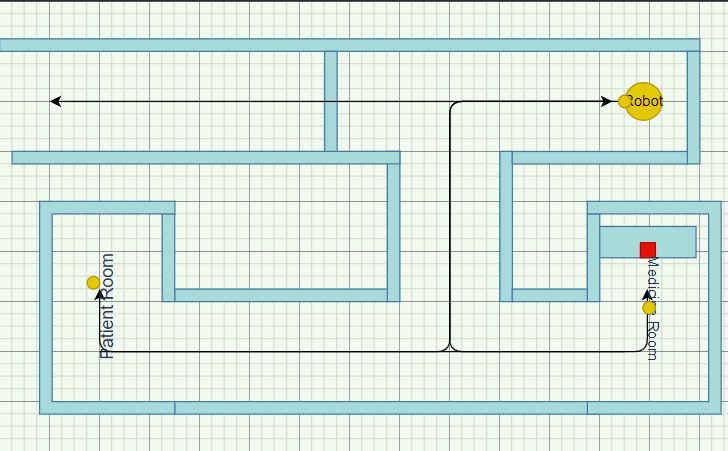
\includegraphics[width=.8\textwidth]{img/map_example.png}
    \caption{Exemplo de mapa de uma simulação}
    \label{fig:example_map}
\end{figure}

\begin{figure}[ht]
    \centering
    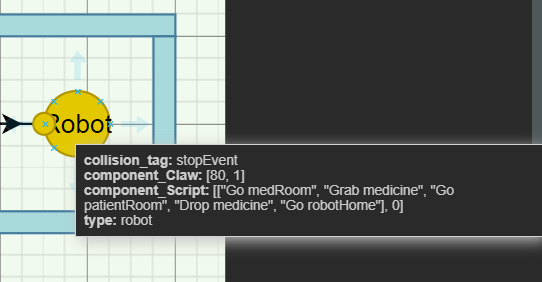
\includegraphics[width=.8\textwidth]{img/robot_annotations.png}
    \caption{Exemplo de anotações em uma entidade}
    \label{fig:example_annotations}
\end{figure}


\section{Arquitetura}
\label{sec:architecture}

\begin{figure}[ht]
    \centering
    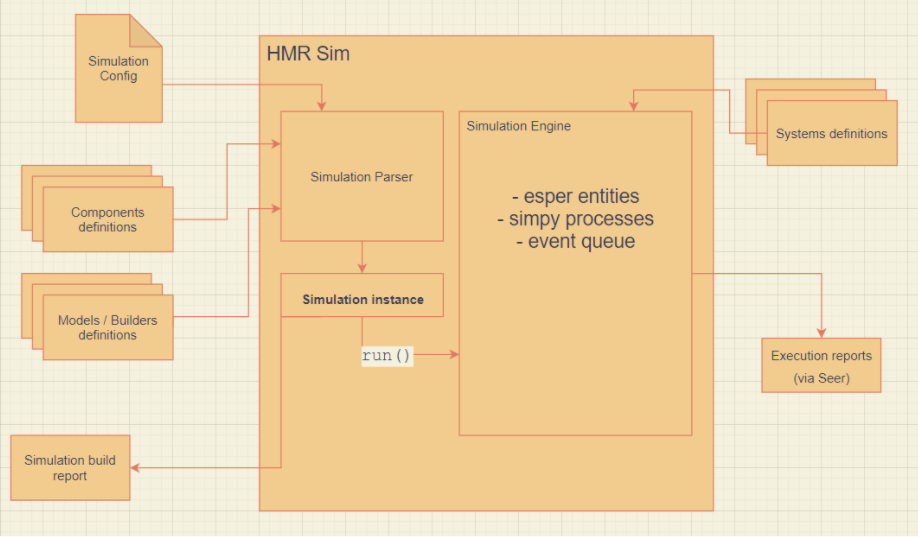
\includegraphics[width=\textwidth]{img/architecture_overview.png}
    \caption{Diagrama representando um resumo da arquitetura do HMR Sim}
    \label{fig:architecture_overview}
\end{figure}

A figura \ref{fig:architecture_overview} mostra um resumo da arquitetura do simulador HMR Sim. A construção da simulação acontece separada da simulação em si. Para construir uma simulação, um objeto de configuração tem que ser passado para o simulador, bem como as definições dos componentes disponíveis e os \texttt{models} e \texttt{builders} disponíveis. A classe \texttt{Simulator} cria a simulação, e depois a executa. A instancia da simulação mostrada na figura \ref{fig:architecture_overview} (\textit{Simulation instance}) é exatamente a instância da classe \texttt{Simulator} criada.

O objeto de configuração é um dicionário Python, que pode ser salvo como um arquivo \texttt{json}. Algumas das opções mais importantes estão listadas abaixo. Para ver todas as opções verifique a documentação do projeto, no repositório.

\begin{itemize}
    \item \textbf{context} (string) - A raíz do projeto, de onde componentes, sistemas e builders extras serão incluídos;
    \item \textbf{map} (string) - O arquivo XML do mapa
    \item \textbf{FPS} (int) - Frequência com que serão executados os sistemas do \texttt{esper}. Esses sistemas não geram eventos, são indicados para representar sistemas que acontecem de forma frequênte e previsível. Caso nenhum sistema \texttt{esper} seja utilizado não é necessário informar esse valor.
    \item \textbf{duration} (int) - Tempo limite da simulação (no relógio da simulação). Por exemplo, um valor 6 vai fazer o simulador encerrar a simulação após 6s serem simulados.
    \item \textbf{simulationComponents} (dict) - Componentes "globais". Eles são adicionados à entidade 1, reservada à simulação. Podem ser acessados por todos os robôs (e.g. um mapa compartilhado de rotas).
    \item \textbf{extraEntities} (EntityDefinition[]) - Lista de \texttt{EntityDefinition} (ver documentação), que definiem entidades que não estão presentes no mapa mas devem ser incluídas na simulação. É possível declarar todas as entidades com essa opção e usar o mapa apenas para coisas estáticas, reaproveitando-o para vários cenários. 
\end{itemize}

O simulador importa automaticamente \texttt{components}, \texttt{models} e \texttt{builders} do sistema de arquivos. Por conta disso os projetos que usem o HMR Sim precisam de uma organização expecífica, como mostrado abaixo. Dentro de cada pasta os arquivos deve estar no formato apropriado.

\dirtree{%
    .1 project\_root.
    .2 models.
    .2 components.
    .2 builders.
}

A simulação construída se torna uma instância da classe \texttt{Simulator} cujo atributo \texttt{World} está preenchido com as entidades que foram criadas, e as opções de configuração salvas. Essa instância é um objeto Python, podendo ser salvo através da biblioteca \texttt{pickle}, por exemplo, e distribuído. Antes de poder ser executada, no entanto, é necessário inicializar e adicionar os sistemas à simulação. Para adicionar sistemas os métodos \texttt{Simulator.add\_system} e \texttt{Simulator.add\_des\_system} podem ser usados. Qual dos dois usar depende do sistema a ser adicionado, detalhes na Seção \ref{sec:systems}.

Após adicionar os sistemas, a simulação pode ser executada utilizando o método \texttt{Simulator.run}, da instância do simulador gerada. A simulação é executada por \texttt{duration} segundos de simulação, se essa opção foi passada na configuração, ou até que o evento \texttt{KILL\_SWITCH} seja processado. É possível manter ver logs da simulação durante a execução. A visualização gráfica da simulação é implementada através do sistema Seer, discutido na seção \ref{sec:seer}.

Alguns sistemas com funcionalidades consideradas essenciais na maior parte das simulações já foram implementados, como parte da validação do simulador. Eles serão detalhados na Seção \ref{sec:systems_available}, e incluem sistema de navegação, movimentação, colisão, controle de robôs, sensores, e visualização.

\section{\texttt{builders} e \texttt{models}}
\label{sec:builders_and_models}

Os arquivos XML que podem ser usados de mapas representam os objetos desenhados dentro de tags \texttt{<mxCell>}, com alguma geometria. Diferentes formas possuem diferentes conteúdos na tag \texttt{<mxCell>}. \texttt{models} são funções que traduzem o XML em uma \texttt{<mxCell>} para uma lista de componentes da simulação. Cada \texttt{model} deve ser armazenado em um arquivo próprio que exporte: (1) uma função \texttt{from\_mxCell}, que recebe uma \texttt{<mxCell>} e retorna uma lista de componentes; (2) uma constante \texttt{MODEL} com o nome da forma que esse model traduz.

\texttt{builders} são semelhantes aos \texttt{models}, mas fazem a tradução do XML contido em \texttt{<object>}. Qualquer forma (\texttt{<mxCell>}) que tenha anotações (como as mostradas na figura \ref{fig:example_annotations}) é envolvida em uma tag \texttt{<object>} que guarda as anotações. \texttt{builders} traduzem tanto as anotações no objeto quanto o XML da \texttt{<mxCell>} contido nele. Eles podem ou não fazer uso de \texttt{models} para isso. UM \texttt{builder} deve estar em um arquivo próprio que exporte: (1) uma função \texttt{build\_object}, que transforma o XML do objeto e (2) uma constante \texttt{TYPE}, indicando que esse \texttt{builder} deve ser aplicado em objetos que tenham a anotação \texttt{type} com esse valor.

Os \texttt{models} e \texttt{builders} são opcionais. Caso todas as entidades sejam criadas através da opção \texttt{extraEntities} da configuração eles serão desnecessários. Atualmente cerca de 10 formas podem ser usadas, e cerca de 7 \texttt{builders} foram criados.

\section{Entidades e Componentes}
\label{sec:ents_and_components}

HMR Sim utiliza a biblioteca \texttt{esper} \cite{esper} (ver detalhes na Seção \ref{sec:ECS}) para gerenciar as entidades e seus componentes na simulação. Cada entidade do mapa ou das entidades passadas pela configuração é representada por um inteiro, armazenado dentro da classe \texttt{World} do \texttt{esper}, e pode ser acessado através da instância da simulação no atributo \texttt{world}, e também pelos sistemas. O identificador de cada objeto do mapa e qual entidade corresponde a ele fica armazenado no atributo \texttt{draw2ent} do simulador. Entidades também podem ser adicionadas diretamente à simulação através do método \texttt{Simulator.add\_entity}.

Entidades possuem um conjunto de componentes. componentes podem ser adicionados ou removidos de entidades usando métodos da biblioteca \texttt{esper}. Existem também métodos para verificar a existência de um componente em uma entidade, buscar componentes específicos de entidades, buscar todos os componentes de um certo tipo no \texttt{World}, etc. Componentes são simplesmente classes Python, que devem ter o mesmo nome que o arquivo que as declara (uma por arquivo). É convencionado no padrão ECS que os componentes não tenham lógica implementada, sugere-se que apenas os métodos \texttt{\_\_init\_\_} e \texttt{\_\_str\_\_} sejam implementados em um componente. \texttt{@dataclass} podem ser utilizadas. 

O identificador de um componente é o nome da sua classe. Dessa forma, se o componente \texttt{simulator.componentes.MyComponent} for declarado, para utilizá-lo em algum sistema pode-se importá-lo normalmente (e.g. \texttt{from simulator.components.MyComponent import MyComponent}) e usar essa importação ao se referir ao componente (buscando-o no \texttt{World}, por exemplo).

\section{Sistemas}
\label{sec:systems}

Sistemas são uma parte essencial do simulador, pois são os responsáveis por fazerem a simulação acontecer. Sistemas são também muito versáteis, podendo ser usados não só para representar uma parte da simulação, mas também para extrair informações dela. Existem 2 tipos diferentes de sistemas que podem ser usados: (1) um sistema compatível com sistemas da biblioteca \texttt{esper}, referidos como "sistemas normais" e sistemas compatíveis com a biblioteca \texttt{simpy}, referidos como "sistemas DES". Ambos são opcionais e o uso de um ou outro depende do que será simulado pelo sistema. As seções \ref{sec:normal_systems} e \ref{sec:des_systems} explicam a diferença entre eles e as particularidades de cada um.

O conceito central do HMR Sim é que sistemas são construídos para utilizar um conjunto de componentes e representar uma parte da simulação. Cada conjunto de sistemas relacionados (e seus componentes) confere novas capacidades ao simulador, e portanto à simulação sendo feita, por exemplo sistemas podem representar sensores, movimentação, comunicação entre robôs, etc. Grande parte da flexibilidade que o simulador proporciona está na relativa facilidade de criar e usar sistemas. Se algum sistema não se adequa às suas necessidades, basta substituí-lo por outro, ou modificá-lo, sem ter que alterar outras partes da simulação. Por exemplo, se o objetivo de uma simulação é comparar dois algoritmos de gerenciamento de robôs, 2 sistemas diferentes (que usem os mesmos componentes) serão criados, um para cada algoritmo. Testar o algoritmo A ou B se torna uma simples questão de adicionar o sistema A ou B na simulação.

\subsection{Sistemas compatíveis com \texttt{esper}}
\label{sec:normal_systems}

Os "sistemas normais" são aqueles que ficam armazenados dentro do \texttt{World} do \texttt{esper}. Eles são definidor como classes que extendem a classe \texttt{esper.Processor} e devem implementar 2 funções: \texttt{\_\_init\_\_} e \texttt{process}. A função \texttt{process} recebe dois argumentos, \texttt{self}, a instância do \texttt{World}  e \texttt{kwargs}, os parâmetros passados pelo \texttt{Simulator} aos sistemas (ver documentação).

Esses sistemas (e apenas eles) são executados pelo \texttt{esper}. Para utilizzá-los é necessário passar a opção \texttt{FPS} na configuração da simulação. Esses sistemas serão então executados uma vez a cada $\frac{1}{FPS}$ segundos de simulação. Note que o uso desses sitemas força a simulação a correr em passos (i.e. o relógio da simulação vai andar em intervalos de, no máximo, $\frac{1}{FPS}$).

Esse tipo de sistema é indicado para simular comportamentos constantes e repetitivos, com frequência definida. Por exemplo movimentação, verificação de colisão, aumento de temperatura em uma sala, gasto de bateria, etc. Eles geralmente seguem o formato mostrado no código \ref{code:normal_system}

\begin{adjustwidth}{-1cm}{0cm}
\lstinputlisting[language=Python, basicstyle=\ttfamily\small, captionpos=b,caption=Formato básico de um sistema normal, label=code:normal_system]{snippets/normal_system_scaffold.py}
\end{adjustwidth}

\subsection{Sistemas compatíveis com \texttt{simpy}}
\label{sec:des_systems}

Os "sistemas DES" são gerenciados pelo \texttt{simpy}. Eles são definidos como processos do \texttt{simpy}, e podem ser qualquer processo aceito pelo \texttt{simpy}, ou seja, qualquer função geradora. Sugere-se, como convenção, usar uma função chamada \texttt{process}. Opcionalmente podem também definir uma função de limpeza, que será executada ao final da simulação, e serve para fechar arquivos que foram abertos, por exemplo. Esses sistemas "vivem" todos dentro do mesmo ambiente do \texttt{simpy}, que é armazenado como um dos atributos da simulação.

A comunicação entre esse tipo de sistema aproveita os eventos suportados pelo \texttt{simpy}, utilizando o recurso \texttt{EVENT\_STORE}, outro atributo do simulador. Convenciona-se que apenas eventos (\texttt{EVENT} ou \texttt{ERROR}, ver \texttt{typehints} na documentação do simulador) sejam utilizados dentro da \texttt{EVENT\_STORE}. Cada sistem pode exportar seu próprio payload e tag para eventos. Assim, qualquer outro sistema que queira enviar uma mensagem para o sistema em questão só precisa criar um novo evento com o payload e tag apropriado e adicioná-lo a \texttt{EVENT\_STORE}. Esse sistema de comunicação permite a criação de sistemas reativos, que apenas processam eventos esperados por eles, e no resto do tempo ficam desativados.

É possível também um sistema em determinado momento criar um canal temporário para aguardar uma resposta de alguma operação asíncrona. É possível também que um sistema execute em mais de uma thread, mas a thread principal deve executar na mesma que o resto do simulador, e deve ser adicionada ao ambiente \texttt{simpy}. A comunicação entre as threads so sistema é de responsabilidade dele.

Durante a execução argumento \texttt{kwargs} é passado aos sistemas, dando acesso ao \texttt{World}, ao ambiente \texttt{simpy} da simulação, à \texttt{EVENT\_STORE}, o evento \texttt{KILL\_SWITCH}, etc. Essas informações permitem ao sistema grande poder sobre a simulação. O evento \texttt{KILL\_SWITCH} é um evento especial que termina a simulação se for disparado.

Esses tipo de sistema é indicado para simular comportamentos inconstantes ou imprevisíveis, sistemas reativos ou ainda como plugins, exetendendo o simulador. O código \ref{code:des_system} representa o formato típico de um sistema DES.

\begin{adjustwidth}{-1cm}{0cm}
    \lstinputlisting[language=Python, basicstyle=\ttfamily\small, captionpos=b,caption=Formato básico de um sistema DES, label=code:des_system]{snippets/des_system_scaffold.py}
\end{adjustwidth}

\section{Sistemas Disponíveis}
\label{sec:systems_available}

\subsection{Seer}
\label{sec:seer}